\documentclass[aspectratio=169]{beamer}

% ---------- ENCODING & FONTS ----------
\usepackage[utf8]{inputenc}
\usepackage[T1]{fontenc}

% ---------- THEME & LOOK ----------
\usetheme{Madrid}
\usecolortheme{seahorse}
\usefonttheme{professionalfonts}
\setbeamertemplate{navigation symbols}{}
\setbeamercovered{transparent}
\setbeamertemplate{itemize items}[circle]
\setbeamertemplate{enumerate items}[default]
\setlength{\parskip}{0.25em}

% ---------- COLORS ----------
\definecolor{accent}{RGB}{0,92,184}
\definecolor{soft}{RGB}{233,244,255}
\definecolor{canadared}{RGB}{196,30,58}
\definecolor{leafgreen}{RGB}{0,130,80}
\definecolor{goldenrod}{RGB}{218,165,32}
\definecolor{deeporange}{RGB}{220,90,20}
\definecolor{shiftpurple}{RGB}{130,50,180}
\definecolor{tealblue}{RGB}{0,128,128}
\definecolor{lightred}{RGB}{245,210,210}
\setbeamercolor{structure}{fg=accent}
\setbeamercolor{title}{fg=white,bg=accent}
\setbeamercolor{frametitle}{fg=accent}
\setbeamercolor{block title}{bg=accent!12,fg=accent}
\setbeamercolor{block body}{bg=soft}

% ---------- PACKAGES ----------
\usepackage{booktabs}
\usepackage{amsmath, amssymb}
\usepackage{array}
\usepackage{multirow}
\usepackage{hyperref}
\usepackage{tikz}
\usepackage{pgfplots}
\pgfplotsset{compat=1.18}
\usetikzlibrary{arrows.meta, positioning, calc, shapes.geometric}
\hypersetup{colorlinks=true,linkcolor=accent,urlcolor=accent}

% ---------- SAFE TRANSITION FALLBACK ----------
\makeatletter
\@ifundefined{transfade}{\newcommand{\transfade}[1][]{}}{}
\makeatother

% ---------- DEGREE SYMBOL ----------
\newcommand{\degree}{$^\circ$}

% ---------- TITLE ----------
\title{\textbf{Aggregate Expenditure and Output in the Short Run}}
\subtitle{{\large ECON 101 -- Principles of Macroeconomics}}
\author{Muhebullah Karimzada}
\date{Spring 2026}

% ============================================================
\begin{document}
% ============================================================

\begin{frame}[plain]
  \titlepage
\end{frame}

\begin{frame}{Chapter Outline}
\transfade
\begin{itemize}[<+->]
  \item \textbf{8.1} The Aggregate Expenditure Model
  \item \textbf{8.2} Determining Aggregate Expenditure in the Economy
  \item \textbf{8.3} Graphing Macroeconomic Equilibrium
  \item \textbf{8.4} The Multiplier Effect
  \item \textbf{8.5} The Aggregate Demand Curve
  \item \textbf{Appendix} The Algebra of Macroeconomic Equilibrium
\end{itemize}
\end{frame}

% ============================================================
\section{8.1 The Aggregate Expenditure Model}
% ============================================================

\begin{frame}{8.1 Learning Objective}
\transfade
\begin{block}{Goal}
Understand how macroeconomic equilibrium is determined in the aggregate expenditure model.
\end{block}
\begin{itemize}[<+->]
  \item We build the \textbf{aggregate expenditure (AE) model}: a short-run model.
  \item It studies the relationship between total spending and output,
  \item \textbf{assuming the price level is constant} in the short run.
  \item Why study this? It helps us understand:
  \begin{itemize}[<+->]
    \item why recessions occur,
    \item why government stimulus can boost the economy,
    \item and how the \textbf{multiplier effect} works.
  \end{itemize}
\end{itemize}
\end{frame}

\begin{frame}{Aggregate Expenditure: Definition}
\transfade
\begin{itemize}[<+->]
  \item \textbf{Aggregate expenditure (AE):} total planned spending in the economy.
  \[
    AE = C + I + G + NX
  \]
  \begin{itemize}[<+->]
    \item $C$: consumption (households buying groceries, cars, Netflix subscriptions)
    \item $I$: planned investment (firms buying machines, households buying new homes)
    \item $G$: government purchases (federal, provincial, municipal)
    \item $NX$: net exports (exports minus imports)
  \end{itemize}
  \item \textbf{Canadian AE composition (2023, Statistics Canada):}
  \begin{itemize}[<+->]
    \item $C \approx 56\%$, $I \approx 21\%$, $G \approx 22\%$, $NX \approx 1\%$ of GDP.
  \end{itemize}
\end{itemize}
\end{frame}

\begin{frame}{Table 8.1 -- Canadian Components of AE (2023)}
\begin{center}
\begin{tikzpicture}
\begin{axis}[
  width=0.70\textwidth, height=0.70\textheight,
  ybar, bar width=1.1cm,
  xlabel={Component of AE},
  ylabel={Share of GDP (\%)},
  symbolic x coords={C,I,G,NX},
  xtick=data,
  ymin=0, ymax=65,
  nodes near coords,
  nodes near coords style={font=\small, anchor=south},
  tick label style={font=\normalsize},
  label style={font=\small},
  title style={font=\small\bfseries},
  title={Canada: Consumption Dominates Aggregate Expenditure},
  enlarge x limits=0.2
]
\addplot[fill=accent!80, draw=accent] coordinates {(C,56)(I,21)(G,22)(NX,1)};
\end{axis}
\end{tikzpicture}
\end{center}
{\tiny Source: Statistics Canada, National Accounts (Table 36-10-0104-01), 2023 estimates.}
\end{frame}

\begin{frame}{Planned vs. Actual Investment}
\transfade
\begin{itemize}[<+->]
  \item National accounts measure \textbf{actual investment}.
  \item AE model uses \textbf{planned investment}: what firms intend to invest.
  \item \textbf{Actual investment} = planned investment + \textbf{unplanned inventory changes}.
  \item \textbf{Why inventories matter:}
  \begin{itemize}[<+->]
    \item If sales are \alert{lower than expected}: inventories build up unintentionally (firms reduce output).
    \item If sales are \alert{higher than expected}: inventories fall unintentionally (firms increase output).
  \end{itemize}
  \item \textbf{Canadian example (2022):} supply chain disruptions left Canadian auto dealers with record-low inventories --- firms scrambled to increase output.
\end{itemize}
\end{frame}

\begin{frame}{Macroeconomic Equilibrium in the AE Model}
\transfade
\begin{itemize}[<+->]
  \item \textbf{Macroeconomic equilibrium:}
  \[
    \text{Planned AE} = \text{Real GDP}
  \]
  \item If planned AE $>$ output:
  \begin{itemize}[<+->]
    \item firms sell more than expected, inventories fall,
    \item firms \alert{increase} production and employment.
  \end{itemize}
  \item If planned AE $<$ output:
  \begin{itemize}[<+->]
    \item firms sell less than expected, inventories rise,
    \item firms \alert{reduce} production and employment.
  \end{itemize}
  \item \textbf{Inventories are the adjustment mechanism} that pushes the economy toward equilibrium.
\end{itemize}
\end{frame}

% ------------------------------------------------------------
% Consumption Function
% ------------------------------------------------------------

\begin{frame}{Determinants of Consumption}
\transfade
\begin{columns}
\column{0.48\textwidth}
\begin{block}{\textcolor{accent}{Increase Consumption}}
\begin{itemize}
  \item Higher disposable income
  \item Higher household wealth (house prices, stock market)
  \item Higher expected future income
  \item Lower interest rates
  \item Higher consumer confidence
\end{itemize}
\end{block}
\column{0.48\textwidth}
\begin{block}{\textcolor{canadared}{Decrease Consumption}}
\begin{itemize}
  \item Lower disposable income
  \item Wealth destruction (market crash)
  \item Pessimistic income expectations
  \item Higher interest rates
  \item Low consumer confidence
\end{itemize}
\end{block}
\end{columns}
\vspace{0.5em}
\begin{itemize}[<+->]
  \item \textbf{Canadian example (2022--2024):} Bank of Canada raised overnight rate from 0.25\% to 5.0\%. This reduced consumer spending, especially on mortgages, autos, and durables --- Canadian consumer confidence fell sharply.
\end{itemize}
\end{frame}

\begin{frame}{The Consumption Function and MPC}
\transfade
\begin{itemize}[<+->]
  \item The \textbf{consumption function}:
  \[
    C = C_0 + \text{MPC} \times Y_D,
  \]
  where:
  \begin{itemize}[<+->]
    \item $C_0$ = autonomous consumption (consumption when $Y_D = 0$),
    \item $Y_D$ = disposable income = $Y - T_{\text{net}}$,
    \item $\text{MPC}$ = marginal propensity to consume.
  \end{itemize}
  \item \textbf{MPC:}
  \[
    \text{MPC} = \frac{\Delta C}{\Delta Y_D}.
  \]
  \item \textbf{Canadian estimate (Statistics Canada):} MPC $\approx 0.75$--$0.80$.
  \begin{itemize}[<+->]
    \item A \$1{,}000 tax rebate $\Rightarrow$ roughly \alert{\$750--\$800} in new spending.
  \end{itemize}
\end{itemize}
\end{frame}

\begin{frame}{Figure 8.1 -- The Consumption Function}
\begin{center}
\begin{tikzpicture}
\begin{axis}[
  width=0.80\textwidth, height=0.70\textheight,
  xlabel={Disposable Income $Y_D$ (\$000s)},
  ylabel={Consumption $C$ (\$000s)},
  xmin=0, xmax=100, ymin=0, ymax=90,
  xtick={0,20,40,60,80,100},
  ytick={0,20,40,60,80},
  grid=major, grid style={dotted,gray!40},
  tick label style={font=\small},
  label style={font=\small},
  title style={font=\small\bfseries},
  title={Consumption Rises with Disposable Income (MPC = 0.8)}
]
% Consumption function: C = 10 + 0.8*Y
\addplot[accent, very thick, domain=0:100] {10 + 0.8*x}
  node[right, font=\small, color=accent] {$C = 10 + 0.8Y_D$};
% 45-degree line (C = Y)
\addplot[gray, dashed, domain=0:90] {x}
  node[right, font=\tiny, color=gray] {$C = Y_D$ (45\degree)};
% Show autonomous consumption C0
\draw[dashed, goldenrod, thick] (axis cs:0,10) -- (axis cs:10,10);
\node[right, font=\tiny, color=goldenrod] at (axis cs:0.5,13) {$C_0=10$};
% Show MPC triangle
\draw[canadared, thick] (axis cs:40,42) -- (axis cs:60,42) -- (axis cs:60,58);
\node[below, font=\tiny, color=canadared] at (axis cs:50,42) {$\Delta Y_D=20$};
\node[right, font=\tiny, color=canadared] at (axis cs:60,50) {$\Delta C=16$};
\node[above, font=\tiny, color=canadared] at (axis cs:52,55) {MPC$=\frac{16}{20}=0.8$};
% Saving annotation
\fill[leafgreen!20] (axis cs:50,50) -- (axis cs:50,10+0.8*50) -- (axis cs:0,0) -- cycle;
\node[font=\tiny, color=leafgreen] at (axis cs:25,28) {Saving $> 0$};
\fill[canadared!20] (axis cs:0,0) -- (axis cs:0,10) -- (axis cs:12.5,10+0.8*12.5) -- cycle;
\node[font=\tiny, color=canadared] at (axis cs:6,7) {Dis-saving};
\end{axis}
\end{tikzpicture}
\end{center}
\end{frame}

\begin{frame}{MPC and MPS}
\transfade
\begin{itemize}[<+->]
  \item \textbf{Marginal propensity to consume (MPC):}
  \[
    \text{MPC} = \frac{\Delta C}{\Delta Y_D}
  \]
  \item \textbf{Marginal propensity to save (MPS):}
  \[
    \text{MPS} = \frac{\Delta S}{\Delta Y_D} = 1 - \text{MPC}
  \]
  \item Every extra dollar of income is either spent or saved:
  \[
    \text{MPC} + \text{MPS} = 1.
  \]
  \item \textbf{Example:} MPC $= 0.8$, so MPS $= 0.2$.
  \begin{itemize}[<+->]
    \item Of an extra \$1{,}000 income: \$800 spent, \$200 saved.
  \end{itemize}
\end{itemize}
\end{frame}

\begin{frame}{Determinants of Planned Investment}
\transfade
\begin{itemize}[<+->]
  \item \textbf{Expectations of future profits:}
  \begin{itemize}[<+->]
    \item Firms invest when optimistic. Recessions reduce planned investment.
    \item \textbf{Canada 2020:} business investment fell $\approx 15\%$ due to pandemic uncertainty.
  \end{itemize}
  \item \textbf{Real interest rate:}
  \begin{itemize}[<+->]
    \item Higher rates $\Rightarrow$ higher cost of borrowing $\Rightarrow$ less investment.
    \item \textbf{Canada 2022--23:} BoC hikes pushed mortgage rates to 6--7\%, residential construction fell sharply.
  \end{itemize}
  \item \textbf{Taxes:}
  \begin{itemize}[<+->]
    \item Higher corporate tax rates reduce after-tax returns on investment.
    \item Canada's federal corporate rate: 15\% (base) + provincial rate.
  \end{itemize}
  \item \textbf{Cash flow:}
  \begin{itemize}[<+->]
    \item Many firms finance investment internally. Lower profits $\Rightarrow$ less cash $\Rightarrow$ less investment.
  \end{itemize}
\end{itemize}
\end{frame}

\begin{frame}{Determinants of Net Exports (NX)}
\transfade
\begin{itemize}[<+->]
  \item \textbf{Net exports} $= $ exports $-$ imports.
  \item Determinants:
  \begin{itemize}[<+->]
    \item \textbf{Relative price levels:} if Canadian prices rise faster than foreign prices, exports fall and imports rise $\Rightarrow$ NX falls.
    \item \textbf{Relative growth rates:} if Canada grows faster than trading partners, imports rise $\Rightarrow$ NX falls.
    \item \textbf{Exchange rate (CAD/USD):}
    \begin{itemize}[<+->]
      \item \alert{CAD appreciates} (CAD strengthens): Canadian exports more expensive for foreigners; imports cheaper $\Rightarrow$ NX falls.
      \item \alert{CAD depreciates} (CAD weakens): Canadian exports cheaper; imports more expensive $\Rightarrow$ NX rises.
    \end{itemize}
  \end{itemize}
  \item \textbf{Canada's key trading partner:} the U.S. takes $\approx$75\% of Canadian exports (Statistics Canada, 2024).
\end{itemize}
\end{frame}

% ============================================================
\section{8.3 Graphing Macroeconomic Equilibrium}
% ============================================================

\begin{frame}{8.3 Learning Objective}
\transfade
\begin{block}{Goal}
Use a 45\degree-line diagram to illustrate macroeconomic equilibrium.
\end{block}
\begin{itemize}[<+->]
  \item Graph \textbf{real GDP} on the horizontal axis.
  \item Graph \textbf{planned aggregate expenditure} on the vertical axis.
  \item The \textbf{45\degree line} shows all points where $AE = Y$ (equilibrium).
  \item The AE line is \textbf{upward sloping} with slope $= $ MPC (since higher $Y \Rightarrow$ higher $C \Rightarrow$ higher AE).
\end{itemize}
\end{frame}

\begin{frame}{Figure 8.2 -- The 45\degree-Line Diagram}
\begin{center}
\begin{tikzpicture}
\begin{axis}[
  width=0.80\textwidth, height=0.72\textheight,
  xlabel={Real GDP ($Y$, \$billions)},
  ylabel={Planned AE (\$billions)},
  xmin=0, xmax=10, ymin=0, ymax=10,
  xtick={0,2,4,6,8,10},
  ytick={0,2,4,6,8,10},
  grid=major, grid style={dotted,gray!40},
  tick label style={font=\small},
  label style={font=\small},
  title style={font=\small\bfseries},
  title={Macroeconomic Equilibrium: Planned AE $=$ Real GDP}
]
% 45-degree line
\addplot[gray, dashed, very thick, domain=0:10] {x}
  node[right, font=\tiny, color=gray] {45\degree\ line ($AE=Y$)};
% AE line (slope = MPC = 0.7, intercept = 2)
\addplot[accent, very thick, domain=0:10] {0.7*x + 2}
  node[right, font=\small, color=accent] {\textbf{AE line}};
% Equilibrium
\addplot[canadared, only marks, mark=*, mark size=4pt] coordinates {(6.67, 6.67)};
\draw[dashed, goldenrod, thick] (axis cs:6.67,6.67) -- (axis cs:6.67,0)
  node[below, font=\small] {$Y^* = \$667B$};
\draw[dashed, goldenrod, thick] (axis cs:6.67,6.67) -- (axis cs:0,6.67)
  node[left, font=\small] {$AE^*$};
% Excess supply annotation
\draw[->, thick, canadared] (axis cs:8.5,8) -- (axis cs:8.5,7.75)
  node[right, font=\tiny, color=canadared, align=left] {$Y > AE$:\\inventories rise,\\firms cut output};
% Excess demand annotation
\draw[->, thick, leafgreen] (axis cs:3.5,3.5) -- (axis cs:3.5,4.45)
  node[right, font=\tiny, color=leafgreen, align=left] {$AE > Y$:\\inventories fall,\\firms boost output};
\node[font=\tiny, fill=white, draw=canadared, rounded corners]
  at (axis cs:6.67,7.5) {\textbf{Equilibrium}};
\end{axis}
\end{tikzpicture}
\end{center}
\end{frame}

\begin{frame}{Understanding the 45\degree Line}
\transfade
\begin{itemize}[<+->]
  \item \textbf{On the 45\degree line:} $\text{Real GDP} = \text{Planned AE}$ --- equilibrium.
  \item \textbf{Above 45\degree line} (AE $>$ Y):
  \begin{itemize}[<+->]
    \item Planned spending exceeds output.
    \item Inventories are depleted.
    \item Firms \alert{increase} production $\Rightarrow$ GDP rises toward equilibrium.
    \item \textbf{Example:} post-COVID reopening 2021 --- consumers spent more than firms produced, pushing GDP higher.
  \end{itemize}
  \item \textbf{Below 45\degree line} (AE $<$ Y):
  \begin{itemize}[<+->]
    \item Planned spending is less than output.
    \item Inventories accumulate unintentionally.
    \item Firms \alert{reduce} production $\Rightarrow$ GDP falls toward equilibrium.
    \item \textbf{Example:} 2020 COVID lockdowns --- businesses produced but few consumers could buy.
  \end{itemize}
\end{itemize}
\end{frame}

% ============================================================
\section{8.4 The Multiplier Effect}
% ============================================================

\begin{frame}{8.4 Learning Objective}
\transfade
\begin{block}{Goal}
Describe the multiplier effect and use the multiplier formula to calculate changes in equilibrium GDP.
\end{block}
\begin{itemize}[<+->]
  \item A small change in \textbf{autonomous expenditure} causes a \textbf{larger} change in equilibrium real GDP.
  \item This amplification is called the \textbf{multiplier effect}.
  \item Why? Because an initial increase in spending raises incomes, which raises consumption, which raises incomes further, and so on.
\end{itemize}
\end{frame}

\begin{frame}{The Multiplier: Step-by-Step}
\transfade
\begin{itemize}[<+->]
  \item Suppose the federal government spends \alert{\$10 billion} on new broadband infrastructure.
  \item \textbf{Round 1:} Telecom workers and contractors receive \$10B income.
  \begin{itemize}[<+->]
    \item They spend $\text{MPC} \times 10 = 0.8 \times 10 = \$8B$ on goods and services.
  \end{itemize}
  \item \textbf{Round 2:} Retailers and service providers receive \$8B.
  \begin{itemize}[<+->]
    \item They spend $0.8 \times 8 = \$6.4B$.
  \end{itemize}
  \item \textbf{Round 3:} $0.8 \times 6.4 = \$5.12B$, and so on...
  \item \textbf{Total effect:} $\Delta Y = 10 + 8 + 6.4 + 5.12 + \ldots = \frac{1}{1-0.8} \times 10 = \alert{\$50B}$.
\end{itemize}
\end{frame}

\begin{frame}{Figure 8.3 -- The Multiplier Effect (MPC $= 0.8$)}
\begin{center}
\begin{tikzpicture}
\begin{axis}[
  width=0.80\textwidth, height=0.70\textheight,
  xlabel={Real GDP ($Y$, \$billions)},
  ylabel={Planned AE (\$billions)},
  xmin=0, xmax=12, ymin=0, ymax=12,
  xtick={0,2,4,6,8,10,12},
  ytick={0,2,4,6,8,10,12},
  grid=major, grid style={dotted,gray!40},
  tick label style={font=\small},
  label style={font=\small},
  title style={font=\small\bfseries},
  clip=false,
  title={$\$1B$ Increase in Autonomous Spending Raises $Y$ by $\$5B$ (Multiplier $= 5$)}
]
% 45-degree line
\addplot[gray, dashed, very thick, domain=0:12] {x};
\node[rotate=45, font=\tiny, color=gray] at (axis cs:9.5,10.0) {$AE=Y$};
% AE1: 0.8Y+1=Y => Y=5
\addplot[accent, very thick, domain=0:11] {0.8*x + 1}
  node[right, font=\tiny, color=accent] {$AE_1$};
% AE2: 0.8Y+2=Y => Y=10
\addplot[leafgreen, very thick, domain=0:11] {0.8*x + 2}
  node[right, font=\tiny, color=leafgreen] {$AE_2$ (+\$1B)};
% Equilibrium 1 at Y=5
\addplot[accent, only marks, mark=*, mark size=3.5pt] coordinates {(5,5)};
\draw[dashed, accent] (axis cs:5,5)--(axis cs:5,0)
  node[below, font=\small, color=accent] {$Y_1=\$5B$};
\draw[dashed, accent] (axis cs:5,5)--(axis cs:0,5)
  node[left, font=\small, color=accent] {$AE_1^*$};
% Equilibrium 2 at Y=10
\addplot[leafgreen, only marks, mark=*, mark size=3.5pt] coordinates {(10,10)};
\draw[dashed, leafgreen] (axis cs:10,10)--(axis cs:10,0)
  node[below, font=\small, color=leafgreen] {$Y_2=\$10B$};
\draw[dashed, leafgreen] (axis cs:10,10)--(axis cs:0,10)
  node[left, font=\small, color=leafgreen] {$AE_2^*$};
% Multiplier annotation below axis
\draw[<->, very thick, deeporange] (axis cs:5,-1.6) -- (axis cs:10,-1.6)
  node[midway, below, font=\small, color=deeporange] {$\Delta Y = \$5B$};
\draw[<->, very thick, shiftpurple] (axis cs:0.4,1) -- (axis cs:0.4,2)
  node[left, font=\tiny, color=shiftpurple, align=right] {$\Delta A$\\$=\$1B$};
\node[font=\small, fill=soft, draw=accent, rounded corners, align=center]
  at (axis cs:3,10) {Multiplier $= \dfrac{1}{1-0.8} = 5$};
\end{axis}
\end{tikzpicture}
\end{center}
\end{frame}

% Cleaner multiplier diagram
\begin{frame}{Figure 8.3b -- Multiplier Effect (Cleaner Illustration)}
\begin{center}

\begin{tikzpicture}
\begin{axis}[
  width=0.80\textwidth, height=0.70\textheight,
  xlabel={Real GDP ($Y$, \$billions)},
  ylabel={Planned AE (\$billions)},
  xmin=0, xmax=14, ymin=0, ymax=14,
  xtick={0,2,4,6,8,10,12,14},
  ytick={0,2,4,6,8,10,12,14},
  grid=major, grid style={dotted,gray!40},
  tick label style={font=\small},
  label style={font=\small},
  title style={font=\small\bfseries},
  clip=false,
  title={Multiplier $= 1/(1-$MPC$) = 1/0.4 = 2.5$ (MPC $= 0.6$)}
]
\addplot[gray, dashed, very thick, domain=0:14] {x};
\node[font=\tiny, rotate=45, color=gray] at (axis cs:11.5,12.2) {$AE=Y$};
% AE1: C=0.6Y+3, I=G=NX gives intercept=3; slope=0.6
\addplot[accent, very thick, domain=0:14] {0.6*x + 3}
  node[right, font=\tiny, color=accent] {$AE_1$ (intercept = \$3B)};
% AE2: shifted up by 2 (autonomous increase of \$2B)
\addplot[leafgreen, very thick, domain=0:14] {0.6*x + 5}
  node[right, font=\tiny, color=leafgreen] {$AE_2$ (+\$2B autonomous)};
% Eq 1: 0.6Y+3=Y => Y=7.5
\addplot[accent, only marks, mark=*, mark size=3.5pt] coordinates {(7.5,7.5)};
\draw[dashed, accent] (axis cs:7.5,7.5)--(axis cs:7.5,0) node[below,font=\small,color=accent]{$Y_1=7.5$};
% Eq 2: 0.6Y+5=Y => Y=12.5
\addplot[leafgreen, only marks, mark=*, mark size=3.5pt] coordinates {(12.5,12.5)};
\draw[dashed, leafgreen] (axis cs:12.5,12.5)--(axis cs:12.5,0) node[below,font=\small,color=leafgreen]{$Y_2=12.5$};
% Multiplier annotation
\draw[<->, very thick, deeporange] (axis cs:7.5,-1.5) -- (axis cs:12.5,-1.5)
  node[midway, below, font=\small, color=deeporange] {$\Delta Y = \$5B$};
\draw[<->, very thick, shiftpurple] (axis cs:7.5,7.5) -- (axis cs:7.5,9.5)
  node[right, font=\tiny, color=shiftpurple, align=left] {Initial\\shift \$2B};
\node[font=\small, fill=soft, draw=accent, rounded corners]
  at (axis cs:4,11) {Multiplier $= \dfrac{\$5B}{\$2B} = 2.5$};
\end{axis}
\end{tikzpicture}
\end{center}
\end{frame}

\begin{frame}{Formula for the Multiplier}
\transfade
\begin{itemize}[<+->]
  \item The total change in equilibrium GDP from an initial change $\Delta A$ in autonomous expenditure:
  \[
    \Delta Y = \Delta A \left[1 + \text{MPC} + \text{MPC}^2 + \text{MPC}^3 + \cdots \right]
            = \frac{1}{1 - \text{MPC}} \times \Delta A.
  \]
  \item \textbf{Multiplier:}
  \[
    \boxed{\text{Multiplier} = \frac{1}{1 - \text{MPC}} = \frac{1}{\text{MPS}}}
  \]
  \item \textbf{Examples:}
  \begin{itemize}[<+->]
    \item MPC $= 0.8$: Multiplier $= \frac{1}{0.2} = 5$.
    \item MPC $= 0.75$: Multiplier $= \frac{1}{0.25} = 4$.
    \item MPC $= 0.5$: Multiplier $= \frac{1}{0.5} = 2$.
  \end{itemize}
  \item \textbf{Real-world multiplier:} much smaller (1.0--1.5) due to taxes, imports, and price changes.
\end{itemize}
\end{frame}

\begin{frame}{The Paradox of Thrift}
\transfade
\begin{itemize}[<+->]
  \item \textbf{Long run:} higher saving $\Rightarrow$ more investment $\Rightarrow$ higher growth.
  \item \textbf{Short run (AE model):} if all households simultaneously save more (consume less):
  \begin{itemize}[<+->]
    \item Consumption falls, AE falls, equilibrium GDP falls.
    \item Could trigger a recession --- even though each individual was being prudent.
  \end{itemize}
  \item This is the \textbf{paradox of thrift}: what is good for individuals can be bad for the economy in the short run.
  \item \textbf{Canadian example (2020):} household saving rate surged to \alert{28\%} during lockdowns.
  \begin{itemize}[<+->]
    \item GDP fell sharply (demand shock).
    \item The ``forced saving'' was then partially spent during the 2021--22 reopening boom.
  \end{itemize}
\end{itemize}
\end{frame}

% ============================================================
\section{8.5 The Aggregate Demand Curve}
% ============================================================

\begin{frame}{8.5 Learning Objective}
\transfade
\begin{block}{Goal}
Understand the relationship between the aggregate demand curve and aggregate expenditure.
\end{block}
\begin{itemize}[<+->]
  \item So far: price level fixed.
  \item Now: what happens to AE when the \textbf{price level changes}?
  \item Three channels link a higher price level to lower AE:
  \begin{enumerate}[<+->]
    \item \textbf{Wealth effect} $\Rightarrow$ lower $C$.
    \item \textbf{Interest-rate effect} $\Rightarrow$ lower $I$.
    \item \textbf{International-trade effect} $\Rightarrow$ lower $NX$.
  \end{enumerate}
  \item A higher price level $\Rightarrow$ lower equilibrium GDP $\Rightarrow$ downward-sloping \textbf{aggregate demand curve}.
\end{itemize}
\end{frame}

\begin{frame}{Figure 8.4 -- From AE to the Aggregate Demand Curve}
\begin{center}
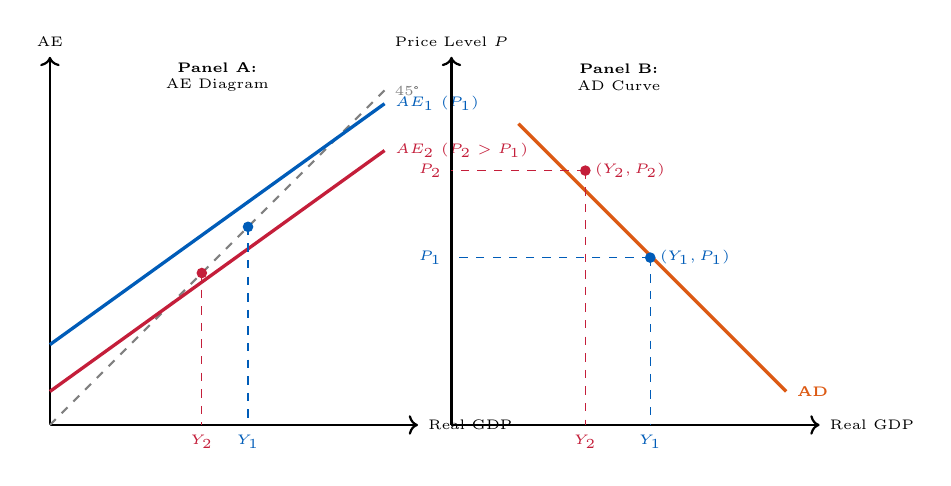
\begin{tikzpicture}[scale=0.85]
% Panel A: AE diagram
\begin{scope}[xshift=-4.5cm]
\draw[->, thick] (0,0) -- (5.5,0) node[right,font=\tiny] {Real GDP};
\draw[->, thick] (0,0) -- (0,5.5) node[above,font=\tiny] {AE};
\draw[gray, dashed, thick] (0,0) -- (5,5) node[right,font=\tiny,color=gray] {45\textdegree};
\draw[accent, very thick] (0,1.2) -- (5,4.8) node[right,font=\tiny,color=accent] {$AE_1$ ($P_1$)};
\draw[canadared, very thick] (0,0.5) -- (5,4.1) node[right,font=\tiny,color=canadared] {$AE_2$ ($P_2>P_1$)};
\draw[dashed,accent] (2.96,2.96)--(2.96,0) node[below,font=\tiny,color=accent] {$Y_1$};
\draw[dashed,canadared] (2.27,2.27)--(2.27,0) node[below,font=\tiny,color=canadared] {$Y_2$};
\filldraw[accent] (2.96,2.96) circle(2pt);
\filldraw[canadared] (2.27,2.27) circle(2pt);
\node[font=\tiny,align=center] at (2.5,5.2) {\textbf{Panel A:}\\AE Diagram};
\end{scope}
% Panel B: AD curve
\begin{scope}[xshift=1.5cm]
\draw[->, thick] (0,0) -- (5.5,0) node[right,font=\tiny] {Real GDP};
\draw[->, thick] (0,0) -- (0,5.5) node[above,font=\tiny] {Price Level $P$};
\draw[deeporange, very thick] (1,4.5) -- (5,0.5)
  node[right,font=\tiny,color=deeporange] {\textbf{AD}};
\filldraw[accent] (2.97,2.5) circle(2pt) node[right,font=\tiny,color=accent] {$(Y_1,P_1)$};
\filldraw[canadared] (2.0,3.8) circle(2pt) node[right,font=\tiny,color=canadared] {$(Y_2,P_2)$};
\draw[dashed,accent] (2.97,2.5)--(2.97,0) node[below,font=\tiny,color=accent] {$Y_1$};
\draw[dashed,canadared] (2.0,3.8)--(2.0,0) node[below,font=\tiny,color=canadared] {$Y_2$};
\draw[dashed,accent] (2.97,2.5)--(0,2.5) node[left,font=\tiny,color=accent] {$P_1$};
\draw[dashed,canadared] (2.0,3.8)--(0,3.8) node[left,font=\tiny,color=canadared] {$P_2$};
\node[font=\tiny,align=center] at (2.5,5.2) {\textbf{Panel B:}\\AD Curve};
\end{scope}
\end{tikzpicture}
\end{center}
\vspace{-0.5em}
{\small Higher price level $\Rightarrow$ AE shifts down $\Rightarrow$ lower equilibrium $Y$ $\Rightarrow$ downward-sloping AD.}
\end{frame}

% ============================================================
\section*{Appendix: Algebra of Macroeconomic Equilibrium}
% ============================================================

\begin{frame}{Appendix -- Solving the AE Model Algebraically}
\transfade
\begin{itemize}[<+->]
  \item Suppose the Canadian economy is described by:
  \begin{align*}
    C &= 400 + 0.8\,(Y - T),\\
    I &= 300,\quad G = 500,\quad T = 250,\quad NX = -50.
  \end{align*}
  \item Equilibrium condition: $Y = C + I + G + NX$.
  \item Substituting:
  \[
    Y = 400 + 0.8(Y - 250) + 300 + 500 - 50.
  \]
  \[
    Y = 400 + 0.8Y - 200 + 750
    \quad \Rightarrow \quad
    0.2Y = 950
    \quad \Rightarrow \quad
    \boxed{Y = \$4{,}750 \text{ billion}}.
  \]
  \item General multiplier: $\frac{1}{1 - \text{MPC}} = \frac{1}{1 - 0.8} = 5$.
\end{itemize}
\end{frame}

% ============================================================
\section*{Chapter Summary}
% ============================================================

\begin{frame}{Summary}
\transfade
\begin{itemize}[<+->]
  \item The \textbf{AE model} determines short-run equilibrium when the price level is fixed.
  \item Equilibrium: $\text{Planned AE} = Y$; inventories adjust to reach this point.
  \item \textbf{Consumption} driven by disposable income (MPC $\approx 0.75$--$0.80$ in Canada), wealth, expectations, and interest rates.
  \item \textbf{Planned investment} driven by profit expectations, interest rates, taxes, and cash flow.
  \item \textbf{Net exports} driven by relative prices, relative growth rates, and the exchange rate.
  \item The \textbf{multiplier} $= 1/(1-\text{MPC})$ amplifies changes in autonomous spending:
  \begin{itemize}[<+->]
    \item Works in both directions --- stimulus boosts GDP, contractionary shock reduces it.
    \item Real-world multipliers are smaller due to taxes, imports, and price changes.
  \end{itemize}
  \item The \textbf{paradox of thrift}: individually rational saving can reduce GDP in the short run.
  \item As the price level changes, AE shifts, tracing out the downward-sloping \textbf{aggregate demand curve}.
\end{itemize}
\end{frame}

\begin{frame}
\centering
\Huge \textbf{Thank you!}\\[1em]
\large Questions?
\end{frame}

\end{document}
